\documentclass[twoside,11pt]{article}
\usepackage[left=1in, right=1in, top=1in, bottom=1in]{geometry}
\usepackage{amsmath}
\usepackage{amssymb}
\usepackage{amsfonts}
\usepackage{mathtools}
\usepackage{amsthm}
\usepackage{fancyhdr}
\usepackage{enumitem}
\usepackage{siunitx}
\usepackage{booktabs}
\usepackage[hidelinks]{hyperref}
\usepackage{sectsty}
\usepackage{mathrsfs} % mathscr
\usepackage{tikz}
\usepackage{pgfplots}
\usepackage{multicol}
\usepackage{listings}
% \usepackage{amsart}

% change mathcal shape
\usepackage[mathcal]{eucal}

% allow H option of figure
\usepackage{float}

% define math operators
\newcommand{\F}{\mathbb{F}}
\newcommand{\R}{\mathbb{R}}
\newcommand{\N}{\mathbb{N}}
\newcommand{\Z}{\mathbb{Z}}
\newcommand{\Q}{\mathbb{Q}}
\newcommand{\X}{\mathbb{Y}}
\renewcommand{\L}{\mathcal{L}}
% \renewcommand{\d}{\mathrm{d}}
\renewcommand*\d{\mathop{}\!\mathrm{d}}
\DeclareMathOperator*{\argmax}{arg\,max}
\DeclareMathOperator*{\argmin}{arg\,min}
\DeclareMathOperator{\im}{im}
\DeclareMathOperator{\id}{id}
\renewcommand{\mod}[1]{\ (\mathrm{mod}\ #1)}

% section font style
\sectionfont{\sffamily\Large}
\subsectionfont{\sffamily\normalsize}
\subsubsectionfont{\bf}

% line spreading and break
\hyphenpenalty=5000
\tolerance=20
\setlength{\parindent}{0em}
\setlength\parskip{0.5em}
\allowdisplaybreaks
\linespread{0.9}

% theorem
% latex theorem
% definition style
\theoremstyle{definition}
\newtheorem{theorem}{Theorem}[subsection]
\newtheorem{axiom}{Axiom}[section]
\newtheorem{definition}{Definition}[section]
\newtheorem{example}{Example}[section]
\newtheorem{question}{Question}[section]
\newtheorem{exercise}{Exercise}[section]
\newtheorem*{exercise*}{Exercise}
\newtheorem{lemma}{Lemma}[section]
\newtheorem{proposition}{Proposition}[section]
\newtheorem{corollary}{Corollary}[section]
\newtheorem*{theorem*}{Theorem}
\newtheorem{problem}{Problem}
% remark style
\theoremstyle{remark}
\newtheorem*{remark}{Remark}
\newtheorem*{solution}{Solution}
\newtheorem*{claim}{Claim}


% paragraph indent
\setlength{\parindent}{0em}
\setlength\parskip{0.5em}

\newcommand\Code{MAT4220 FA22}
\newcommand\Ass{HW\#01}
\newcommand\name{Haoran Sun}
\newcommand\mail{haoransun@link.cuhk.edu.cn}

\title{{\sffamily \Code \ \Ass}}
\author{\sffamily \name \ (\href{mailto:\mail}{\mail})}
\date{\sffamily \today}

\makeatletter
% \let\Title\@title
\let\theauthor\@author
\let\thedate\@date

\fancypagestyle{plain}{%
    \fancyhf{}
    \lhead{\sffamily \Ass}
    \rhead{\sffamily \name}
    \rfoot{\sffamily\thepage}

    % # 页脚自定义
    \fancyfoot[L]{
        \begin{minipage}[c]{0.06\textwidth}
            \includegraphics[height=7.5mm]{logo2.png}
        \end{minipage}
    }
}
\fancypagestyle{title}{%
    \fancyhf{}
    \renewcommand{\headrulewidth}{0pt}
    % \lhead{\Title}
    % \rhead{\theauthor}
    \rfoot{\sffamily\thepage}

    % # 页脚自定义
    \fancyfoot[L]{
        \begin{minipage}[c]{0.06\textwidth}
            \includegraphics[height=7.5mm]{logo2.png}
        \end{minipage}
    }
}
\fancyfootoffset[L]{0.3cm}

% re-define title format
\makeatletter
\renewcommand{\maketitle}{\bgroup\setlength{\parindent}{0pt}
\begin{flushleft}
  \textbf{\Large\@title}

  \@author
\end{flushleft}\egroup
}
\makeatother

\pagestyle{plain}

% lstlisting settings
\lstset{
    basicstyle=\linespread{0.7}\footnotesize,
    breaklines=true,
    basewidth=0.5em
}


\begin{document}
\maketitle
\thispagestyle{title}
% \begin{multicols*}{2}

% \begin{remark}
%     $V_\epsilon(x)$ is used to denote a $\epsilon$-neighborhood
%     \begin{align*}
%         V_\epsilon(x) = B_\epsilon(x)\setminus\{x\}
%     \end{align*}
% \end{remark}

\begin{problem}[P5 Q3]\
\begin{enumerate}[label=(\alph*)]
    \setcounter{enumi}{1}
    \item Second-order linear homogeneous, since the equation $\mathcal{L}u = g$ has
    \begin{align*}
        \mathcal{L} = \partial_t - \partial_{xx} + x
    \end{align*}
    which is a linear operator and $g=0$.
    
    \item Third-order nonlinear, since there is a $uu_x$ term.
    
    \item Second-order linear nonhomogeneous, since the operator
    \begin{align*}
        \L = \partial_{tt} - \partial_{xx}
    \end{align*}
    while $g=-x^2\neq 0$.
    
    \setcounter{enumi}{7}
    \item Forth-order nonlinear, since there is a $\sqrt{u+1}$ term.
\end{enumerate}
\end{problem}

\begin{problem}[P10 Q3]
Note that the set of characteristic curve $h(x, y)=c$
has the properties that 
\begin{align*}
    \frac{\d y}{\d x} = \frac{1}{1+x^2}
\end{align*}
Then we have
\begin{align*}
    y = \arctan x + C
\end{align*}
Then 
\begin{align*}
    u(x,y) = g(C) = g(y-\arctan x)
\end{align*}
Sketch of the characteristic curves:
\begin{figure}[H]
    \centering
    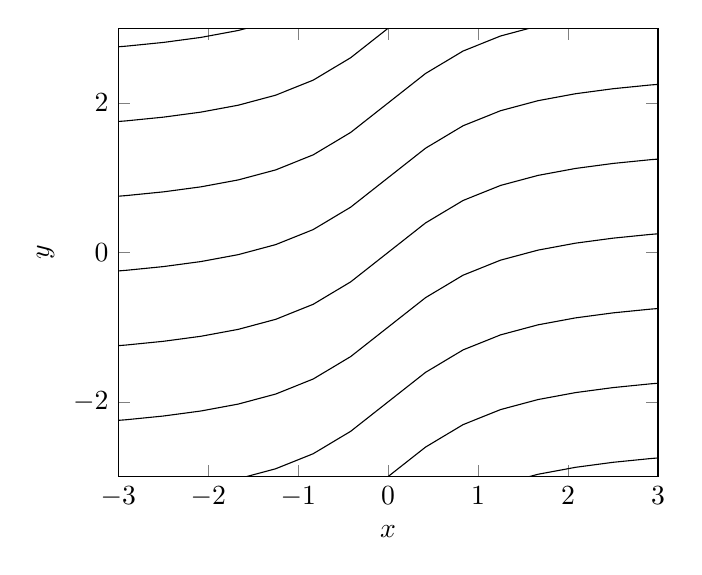
\begin{tikzpicture}
        \begin{axis}[
            ymin=-3, ymax=3, xmin=-3, xmax=3,
            xlabel=$x$, ylabel=$y$
        ]
        \addplot[mark=none]{rad(atan(x))};
        \addplot[mark=none]{rad(atan(x))-1};
        \addplot[mark=none]{rad(atan(x))-2};
        \addplot[mark=none]{rad(atan(x))-3};
        \addplot[mark=none]{rad(atan(x))-4};
        \addplot[mark=none]{rad(atan(x))+1};
        \addplot[mark=none]{rad(atan(x))+2};
        \addplot[mark=none]{rad(atan(x))+3};
        \addplot[mark=none]{rad(atan(x))+4};
        \end{axis}
    \end{tikzpicture}
\end{figure}
\end{problem}

\begin{problem}[P10 Q7]\
\begin{enumerate}[label=(\alph*)]
    \item Characteristic curve satisfies
    \begin{align*}
        \frac{\d y}{\d x} = \frac{x}{y}\Rightarrow x^2 - y^2 = C
    \end{align*}
    Then
    \begin{align*}
        u(x,y) = g(x^2 - y^2)
    \end{align*}
    Plug in $u(0, y) = g(-y^2) = e^{-y^2}$, we have $u(x,y) = e^{x^2 - y^2}$.

    \item Whole $xy$ plane.
\end{enumerate}
\end{problem}

\begin{problem}[P10 Q10]
Change the variable by
\begin{align*}
    x' &= x + y\\
    y' &= -x + y
\end{align*}
Then $u_x=u_{x'}-u_{y'}$, $u_y=u_{x'}+u_{y'}$, and therefore
\begin{align*}
    u_x + u_y + u= 2u_{x'} + u = e^{(3x'+y')/2}
\end{align*}
Solve the homogeneous case $u_{x'}+u=0$, we get kernel $\phi(x',y')$
\begin{align*}
    \phi(x',y')=C(y')e^{-x'/2}
\end{align*}
Suppose a specific solution of the equation is in the form 
\begin{align*}
    u(x',y') = ae^{(3x'+y')/2} + bx'e^{(3x'+y')/2}
\end{align*}
Easy to obtain that $a=1/4$.
Then the general solution of the equation would be
\begin{align*}
    u(x,y) = \frac{1}{4}e^{(3x'+y')/2} + C(y')e^{-x'/2}
    =\frac{1}{4}e^{x+2y} + C(-x+y)e^{-(x+y)/2}
\end{align*}
Apply the boundary condition $u(x,0)=0$, we get
\begin{align*}
    u(x,0) = \frac{1}{4}e^{x} + C(-x)e^{-x/2} = 0\Rightarrow
    C(x)=-\frac{1}{4}e^{-3x/2}
\end{align*}
Then our solution would be
\begin{align*}
    u(x,y) = \frac{1}{4}e^{x+2y} - \frac{1}{4}e^{x-2y}
\end{align*}
\end{problem}

\begin{problem}[P28 Q5]\
    \begin{enumerate}[label=(\alph*)]
        \item Let $y=0$, then we have
        \begin{align*}
            u_{x}(x, 0) = \phi'(x) = 0
        \end{align*}
        this contradicts with the boundary condition $u(x,0)=\phi(x)=x$ since
        \begin{align*}
            \phi'(x) = 1 \neq 0
        \end{align*}
        Therefore, there is no solution.

        \item Applying the technique of characteristic curve, we know that
        $u(x,y)$ is in the form of
        \begin{align*}
            u(x, y) = f(ye^{-x})
        \end{align*}
        Applying the boundary condition, we have
        \begin{align*}
            u(x,0) = f(0) = 0
        \end{align*}
        There are different $f=f(x)$ satisfies $f(0)=0$.
        Then there are multiple solutions.
    \end{enumerate}
\end{problem}

\begin{problem}[P31 Q1]
    \begin{enumerate}[label=(\alph*)]\
        \item The equation is $u_{xx} -4u_{xy} + u_{yy} + 4u = 0$
        \begin{align*}
            A = \begin{bmatrix}
                1 & -2\\
                -2 & 1
            \end{bmatrix}
        \end{align*}
        Since $\det A < 0$, the equation is hyperbolic.

        \item Since
        \begin{align*}
            A = \begin{bmatrix}
                9 & 3\\
                3 & 1
            \end{bmatrix}
        \end{align*}
        and $\det A = 0$, the equation is parabolic.
    \end{enumerate}
\end{problem}

% \end{multicols*}
\end{document}

